\section{Device Drivers}

\subsection{Timer Device}


\noindent
The two main purposes of the timer device is track the time
elapsed since booting and to provide the ability for timeout
callbacks to be registered. 
\\

\noindent
Our timer stores timeouts as a
linked list structure sorted in ascending order of when each
timeout will occur. We choose this data structure as the cost
of removing timeouts from the queue in the IRQ handler is
minimized. The nodes in the linked list are malloc'd from the
heap, but instead of freeing the nodes in the IRQ handler, 
we add them to a free list to be freed (or reused) in subsequent
calls to register new timeouts. This is again done in order to 
minimize the work done in the IRQ handler.
\\

\noindent
Since there are multiple system threads that may simultaneously
access the timer device, we use a notification object in order
to provide exclusive access to critical sections of the device code. Since
the callback functions in timeouts may call into the timer device
themselves (to register another callback for example) our implementation
will safely release the lock to the timer device before executing callbacks,
and re-acquire the lock afterwards.
\\

\noindent
When invoked, our IRQ handler will call as many callbacks as it can
and then program the timer device to create another interrupt when 
the next timeout occurs. Our code will choose the best timer frequency
depending on how far in the future the earliest timeout occurs, so it
is a tickless timer to the extent that is permitted by its limited size. 
The countdown timer is also reprogrammed when new timeouts are registered
and when a callback is removed.
\\

\begin{figure}[h]
    \centering
    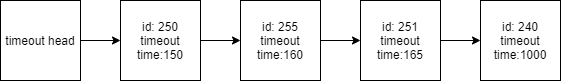
\includegraphics[width=\linewidth]{id_allocation.png}
    \caption{ID allocation example}
    \label{fig:id_allocation}
\end{figure}

\noindent
Our scheme for allocating ids is relatively simple. Ids are allocated in ascending
order, and we have a strategy for wraparound when the maximum assignable id is given.
For example if the size of the id variable is 1 byte and the last id assigned to a 
timeout was 255, then our timer will find the minimum assigned id by iterating
through the list of currently registered callbacks and then start assigning ids 
in descending order from the id before the minimum assigned id. In the situation
depicted above, the minimum assigned id is 240, so the next timeout registered would get
an id of 239, and allocation would continue downward.
\\

\noindent
A similar thing
happens when the value reaches 0 again, the maximum assigned value is found and
id assignment continues upward from there. Given the size of the id field in timeouts
is 32 bits, this 'turnaround' operation will almost never need to be invoked in 
normal usage, and id assignment will occur in amortized constant time. There are
some cases where this will fail, but such cases require extremely large timeout
values and registering callbacks at a high frequency for a long period of time,
situations unlikely to occur during normal usage of SOS.